\chapter{Envelope house model analogous to a 2R-2C network}

The 2R-2C house model structure is implemented as described below:
	
\begin{figure}[H]
	\centering
	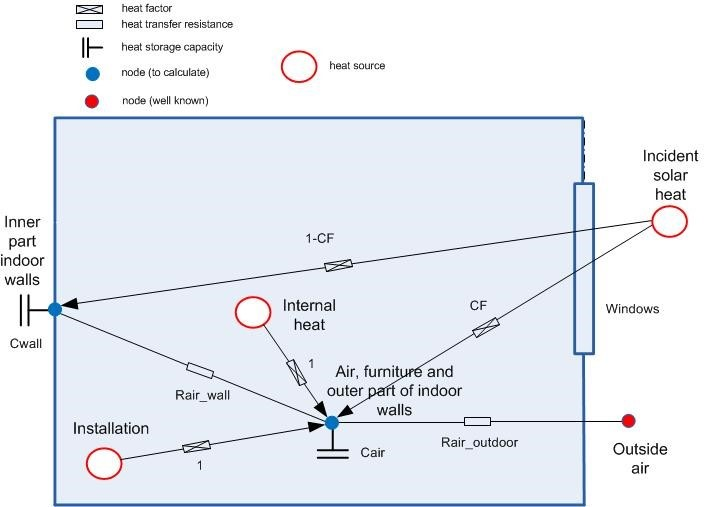
\includegraphics[width=1.0\columnwidth]{Pictures/envelopRC.jpg}
	\caption[Short title]{Schematic of envelope model}
	\label{fig:envelope2R2C}
	\end{figure} 
	
The equivalent electrical 2R-2C network with components and topology is given in Fig. \ref{fig:elec2R2C}.

\begin{figure}[H]
	\centering
	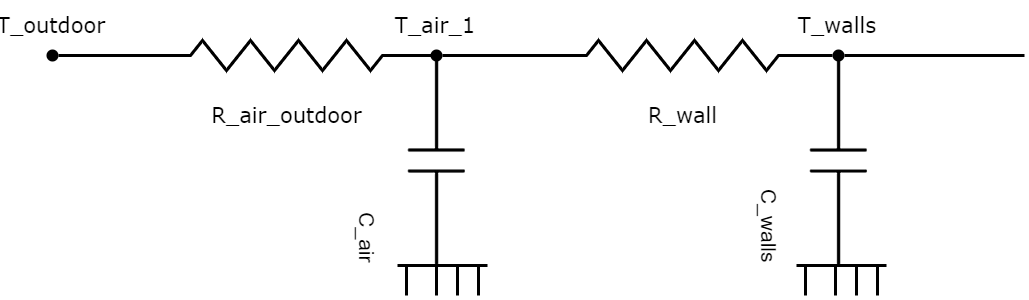
\includegraphics[width=1.0\columnwidth]{Pictures/2R2C_Model.png}
	\caption[Short title]{2R-2C house model}
	\label{fig:elec2R2C}
	\end{figure}
	
The model consists of two capacitances C\textsubscript{air, indoor} and C\textsubscript{wall} and two resistances R\textsubscript{wall} and R\textsubscript{air, outdoor}. The incident solar energy is divided between C\textsubscript{wall} and C\textsubscript{air} through the convection factor CF. It is assumed that both internal heat (lighting, occupancy and electric devices) and supplied heat (installation) initially het up the indoor air. In Fig. \ref{fig:elec2R2C}, they are fully released at the T\textsubscript{air} node. 

